\subsection{Objective and initial conditions} \label{sec:exp-init}
	\begin{figure}[H]
		\centering
		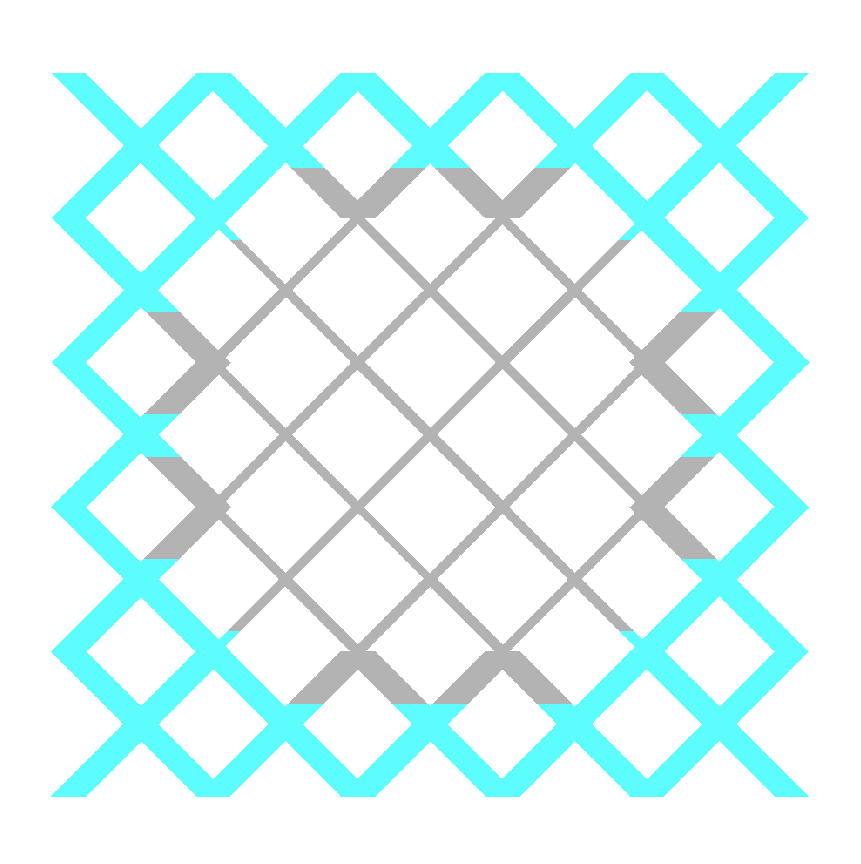
\includegraphics[height=8cm]{fig_result10by10_1}
		\caption{Initial setup example, non-wetting fluid initially located in the region with thinner radii.}
		\label{fig:invasion-result1}
	\end{figure}	
	
	Our objective is to model imbibition. In figure \label{fig:invasion-result1}, all of the wetting fluid is located in the outer region, which has thicker radius. The inner region is filled with non-wetting fluid. In this simulation we wish to analyze the saturation of cyan fluid in the inner region with respect to time, $S = S(t)$. The features of the system are:
	
	\begin{itemize}
		\item The boundaries are closed.
		\item The radius in the outer region is 3 times larger, $R_{outer} = 3 * R_{inner}$.
		\item The size of the system is 26 x 26 tubes.
		\item Initially the volumes of wetting and non-wetting fluids in the whole system are equal. $V_{w} = V_{nw}$
	\end{itemize}
	
\subsection{Experiment (similar thickness)} \label{sec:exp-main}
	The algorithm was implemented in C++ 17, compiled using gcc 9.4.0. The computation was performed using processor 11th Gen Intel Core i5-1135G7 @ 2.40GHz operating with Ubuntu 20.04 LTS. The program was not paralleled, hence only one core of the processor was used at a time. The simulation was done for 20,000 steps. Visualization of meniscus configuration and a plot point of saturation $S(t)$ was made for every 200 steps. It took about 1 minute to compile the whole program, and 5 minutes to simulate. If only the radius or initial meniscus configurations are changed, then recompiling is not required. The node located in the center of the system was chosen to have zero pressure. It was observed that changing the node which will have 0 pressure does not change the geometry of the flow.
	
	\begin{figure}[H]
		\centering
		\begin{subfigure}{0.46\textwidth}
			\centering
			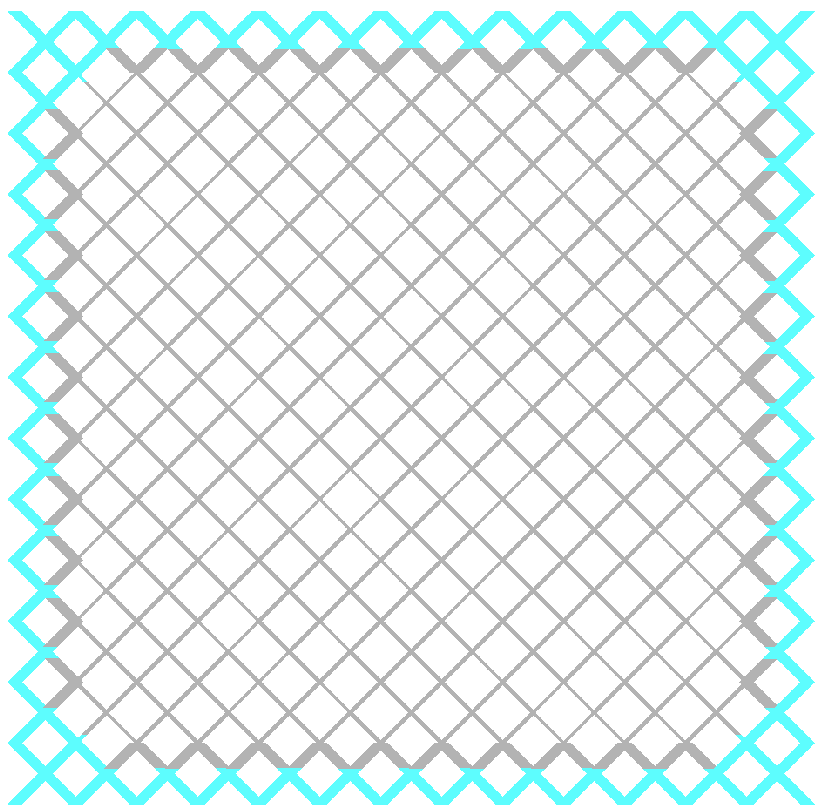
\includegraphics[width=\textwidth]{fig_result26by26_1}
			\caption{Initial setup}
		\end{subfigure}
		\begin{subfigure}{0.46\textwidth}
			\centering
			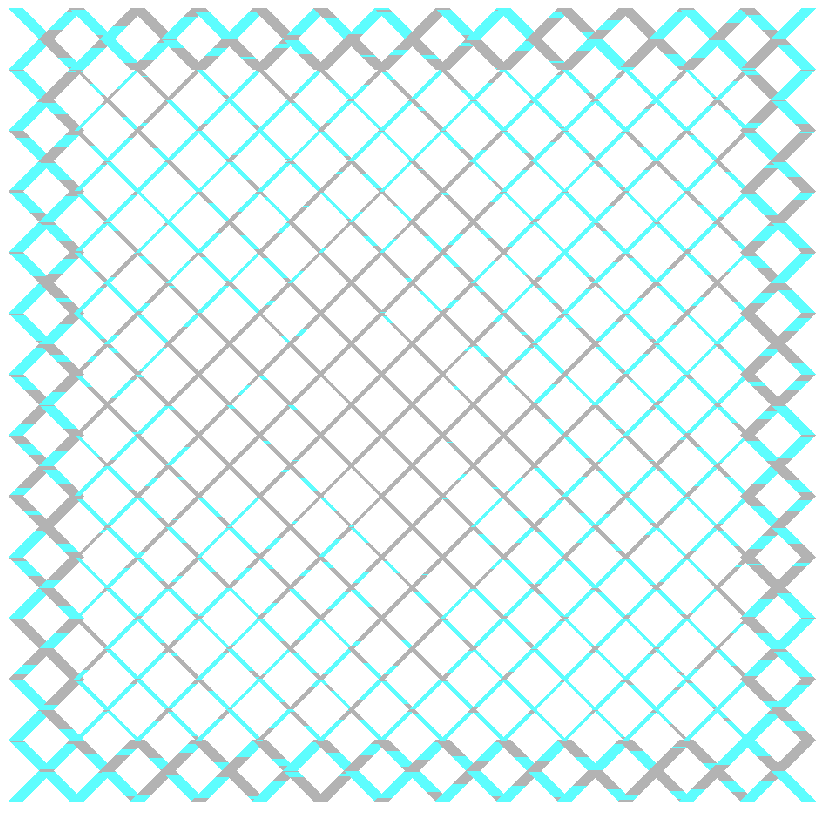
\includegraphics[width=\textwidth]{fig_result26by26_4}
			\caption{Final, in state of equilibrium}
		\end{subfigure}
		\caption{Plots of main experiment}
	\end{figure}
	
	The plots are not symmetric because small random values $\Delta R / R ~ 10^{-3}$ was introduced to the system. The cyan fluid has invaded from the corners. We decided to plot for $26 x 26$ because a network model of this size can be easily simulated on a personal computer in a short time, and also it satisfies the conditions of gray and cyan fluids having about equal volumes, and the inner radius being 3 times thinner than the outer radius.
	
	The the part of the program slowing down the simulation is the solution of the linear equations using Gaussian-elimination. The process of Gaussian-elimination was not optimized. Hence, if we have $m$ variables, the time complexity for solution is $m^3$. If our network model is of size $n x n$ tubes, then the number of nodes is in the order of $n^2$. Therefore the time to compute grows with the size of the network model in the order of $n^6$. If we doubled the size of the network model, it would take $2^6 = 64$ times longer to perform the same simulation, which is about 5 hours on a personal computer, still reasonable time.
	
	For implementing the algorithm, $double$ is recommended over $float$. $float$ was earlier used to speed up the process by about $2$ times, however the errors grew significantly. The saturation is supposed to remain same due to closed boundaries, but it differed by as much as $10\%$ by the end of the simulation. The error in terms of volume of one of the fluid differing was less than $1\%$ when $double$ was used.
	
\subsection{Discussion (similar thickness)} \label{sec:exp-discussion}
	\begin{figure}[H]
		\centering
		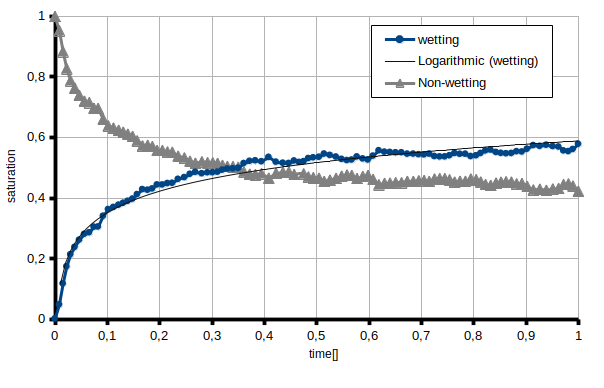
\includegraphics[width=0.7\textwidth]{fig_plot-sat-vs-time2}
		\caption{Plot of saturation of cyan fluid in inner region with respect to dimensionless time.}
	\end{figure}
	
	The equilibrium saturation for wetting fluid, $S_{eq} = 0.57$ for the inner region. For different viscosity ratio ${\mu}_1 / {\mu_2}$, the shape of the plot of $S(t)$ does not significantly differ. Changing constants of the experiment such as $\mu, \sigma, l$ simply changes the scale of the $x-axis$. Since the experiment was not calibrated to actual values, we decided to present our result in dimensionless time. It is obtained by simply diving the values on the $x-axis$ by the maximum.
	
	In in $S(t)$ plot of cyan fluid in the inner region. Initially the rate of invasion accelerates at a high rate, then the acceleration slows down, and finally the saturation reaches an equilibrium value which shows only irregular small oscillations. These irregular oscillations is expected to disappear on using a larger network model. They occur to the blocks of wetting fluid remaining in the outer region.
	
	The invasion of cyan fluid occurred from the corners, because in the corners each node is subjected to capillary forces more than from the middle of the edges. And the gray fluid was pushed out from the middle of the edges. The flow stops because of a large number of tubes ending up with 2 menisci. Tubes with two meniscus have a zero net capillary pressure, and cannot initiate flows. 
	
	$S(t)$ approximately shows a logarithmic dependence. It is clear that the relaxation parameter $\xi$ can be applied here the saturation converges to an equilibrium value.

\subsection{Experiment (varying thickness)}
	In the previous experiment very slight difference in average capillary pressure is observed when the final saturation of wetting fluid is changed in the inner region. 10 experiments were conducted on 30 x 30 networks with varying radii in the inner region. The initial saturation of the wetting fluid was increased by increasing the proportion of wetting fluid in the inner region. Experiment 2- 10 was done for 10,000 steps. Experiment 1 for 3400 steps and experiment 2 for 1000 steps. This is because in experiment 1 - 2, at some moment complete equilibrium was achieved. There were no tubes with odd number of meniscus remaining in the system, therefore no capillary pressure to drive the flow.
	
	The average capillary pressure at the end is calculated by taking the average of $P_c$ according to equation \ref{eq:average-capillary-pressure} in the last 2000 steps of computation for experiments 2 - 10. Averaging was done to smoothing the effects of the vibrations observed in the capillary pressure. However for experiments 1 – 2, the capillary pressure is not the average of some steps, but for the 1000th step and the 3400th step respectively.
	
	Note that at the step when the experiment was forced to be terminated, capillary pressure cannot be defined. Since the total area in the denominator is zero. Radii of {2, 3, 4, 5} +- 0.01 was used in the inner region. Radius of 6 +- 0.01 was used in the outer region. The outer region was approximately half of the total volume.
	
	Also, it was compulsory to add or substract 0.01 randomness to the radius distributions, because in lower initial saturation of blue fluid in the system, a flow will not start.
	
	\begin{figure}[H]
		\centering
		\begin{subfigure}{0.46\textwidth}
			\centering
			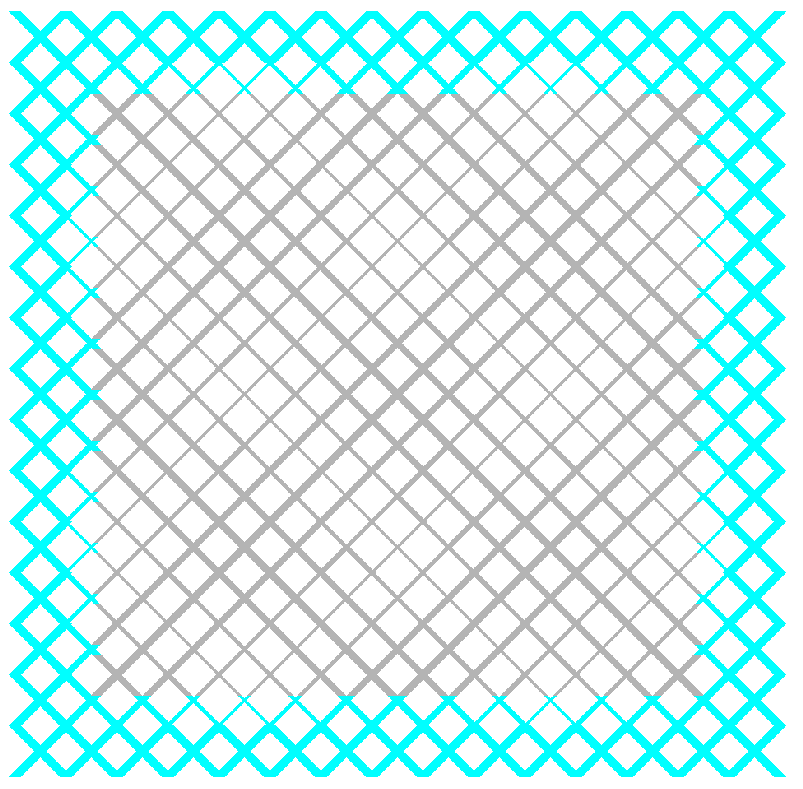
\includegraphics[width=\textwidth]{201-initial-exp}
			\caption{Initial setup}
		\end{subfigure}
		\begin{subfigure}{0.46\textwidth}
			\centering
			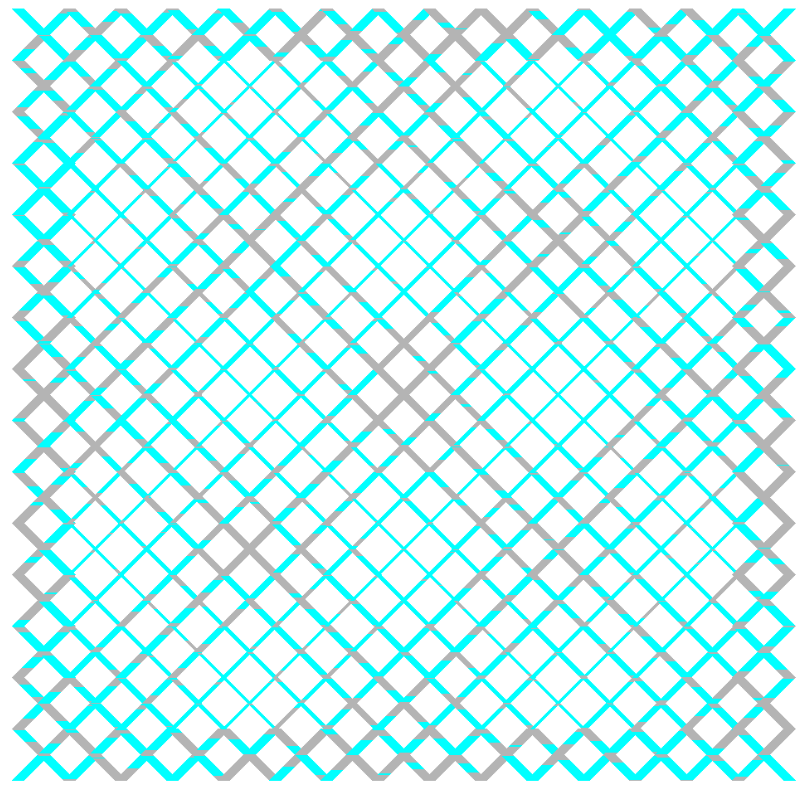
\includegraphics[width=\textwidth]{202-final-exp}
			\caption{Final, in state of equilibrium}
		\end{subfigure}
		\caption{Plots of experiment with varying thickness of tubes in the inner region. It can be seen that since it results in total lower energy of the system, it is more frequent to observe that the wetting fluid occupies the thinner tubes than the thicker tubes.}
	\end{figure}
	
	\begin{figure}[H]
		\centering
		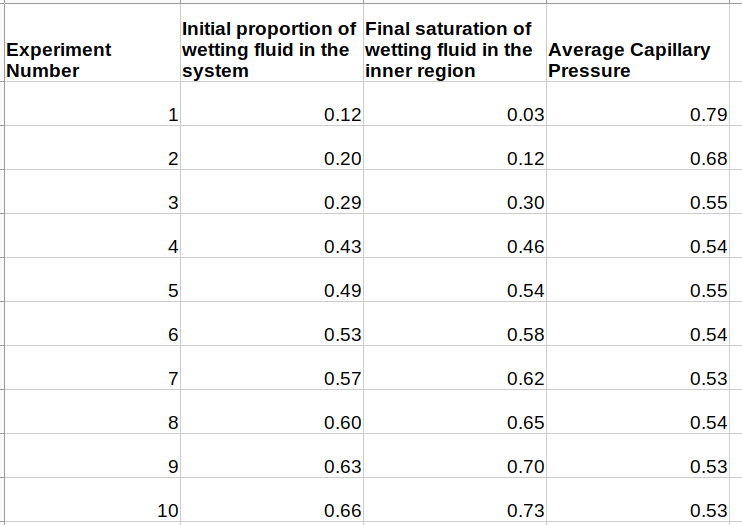
\includegraphics[width=0.6\textwidth]{210-exp-2-table}
		\caption{Experiments conducted, with measurements on the average capillary pressure, initial amount of wetting fluid in the system, final saturation of wetting fluid in the inner region. Note that the final saturation of wetting fluid in the inner region increases with the increase of wetting fluid in the initial conditions.}
		\label{fig:210-exp-2-table}
	\end{figure}
	
	\begin{figure}[H]
		\centering
		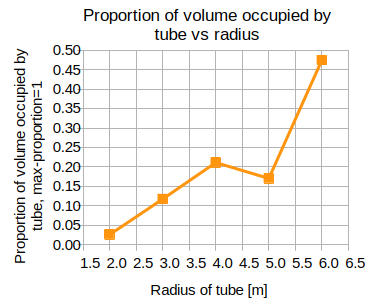
\includegraphics[width=0.6\textwidth]{203-volume-occupied-by-different-radii}
		\caption{showing the relative volume occupied by different groups of tubes with different radii. The average capillary pressure is mainly influenced by the thinnest tubes, therefore we see that the final saturation of the wetting fluid in the inner region must be in the order of the volume of the thinnest tube in order to observe significant changes in the average capillary pressure. }
		\label{fig:203-volume-occupied-by-different-radii}
	\end{figure}
	
	\begin{figure}[H]
		\centering
		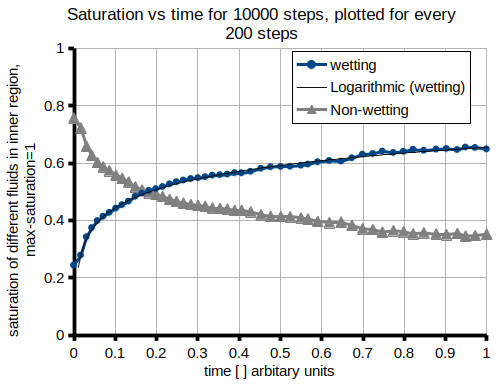
\includegraphics[width=0.8\textwidth]{204-saturation-vs-time}
		\caption{showing that even with varying radii in the inner region, the saturation change with respect to time remains fairly smooth.}
		\label{fig:204-saturation-vs-time}
	\end{figure}
	
	\begin{figure}[H]
		\centering
		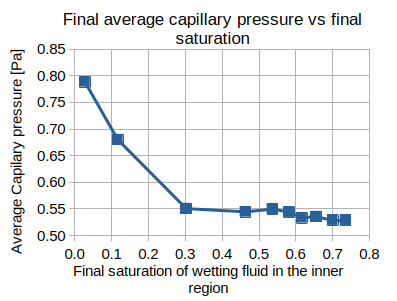
\includegraphics[width=0.6\textwidth]{205-average-capillary-pressure}
		\caption{The average capillary pressure rapidly increases with the decrease in final saturation of wetting fluid in the inner region for very low saturations.}
		\label{fig:205-average-capillary-pressure}
	\end{figure}
	
	\begin{figure}[H]
		\centering
		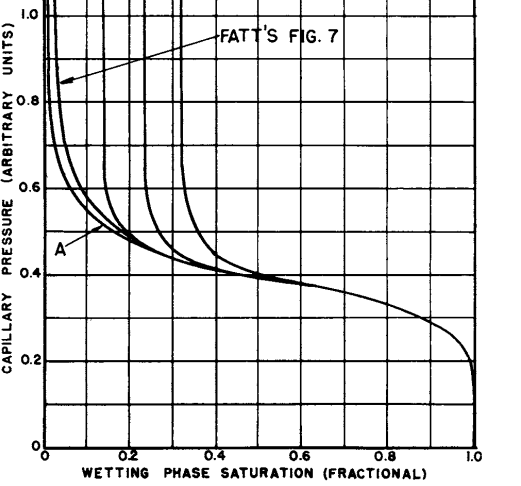
\includegraphics[width=0.4\textwidth]{206-main-reference}
		\caption{the dependence of capillary pressure with saturation of wetting fluid as predicted by Fratt \cite{fatt1956network}}
		\label{fig:206-main-reference}
	\end{figure}

	\begin{figure}[H]
		\centering
		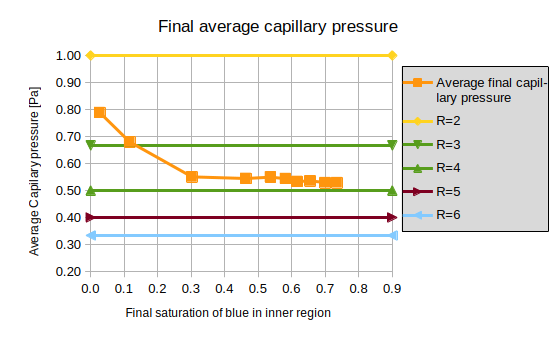
\includegraphics[width=0.95\textwidth]{207-cap-pressure-tube}
		\caption{Capillary pressures in tubes of various radii denoted by horizontal straight lines, and plots of capillary pressures for various final saturations of wetting fluid in the inner region. Clearly the average caoillary pressure is situated in between the maximum and minimum horizontal bars.}
		\label{fig:207-cap-pressure-tube}
	\end{figure}
	
	\begin{figure}[H]
		\centering
		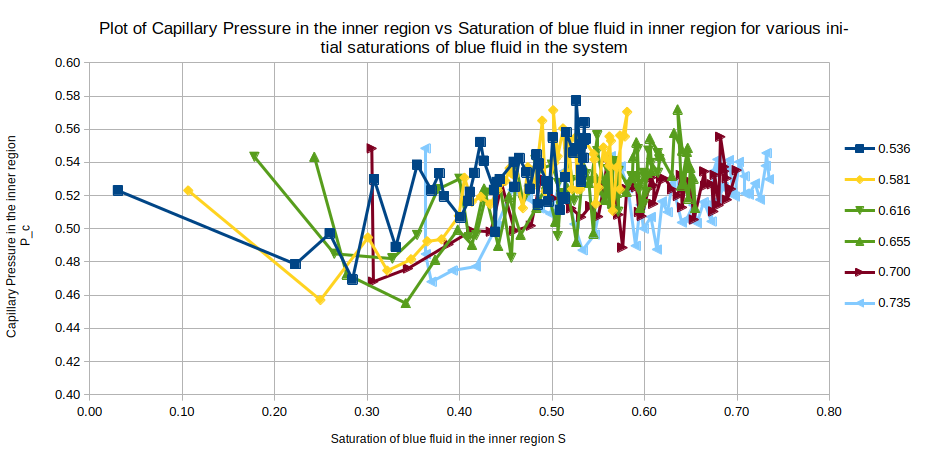
\includegraphics[width=1.0\textwidth]{208-cap-pressure-for-different-experiments}
		\caption{Capillary pressure and saturation points for every 200 steps, for high final saturation of wetting fluid in the inner region. We see that the plots tends to end similarly, however has drastically different initial capillary pressure due to the number of single menisci thinner tubes increased.}
		\label{fig:208-cap-pressure-for-different-experiments}
	\end{figure}

\subsection{Discussion (varying thickness)}
	The final average capillary pressure increased with decreasing the final saturation of wetting (cyan) fluid in the inner region. However since overall less number of meniscus is created in the system is less, we face steps in the experiment where the there is no odd number of meniscus in any tube, and therefore no capillary pressure to continue flow. Therefore for lower than 0.35 initial proportions of blue fluid in the system, the experiment was required to be stopped after a certain number of steps. Since the values of Capillary pressure varied greatly between the 200 steps at which the measurement was recorded, an average of 1000 steps could not be made, therefore further investigation is required to be sure about the increase in capillary pressure.
